\documentclass{beamer}
\usetheme{Manchester}

\usepackage{hyperref}

\newtheorem{remark}[theorem]{Remark}
\newtheorem{caveat}[theorem]{Caveat}
\newtheorem{rmcorollary}[theorem]{Corollary}

\begin{document}

\title[Unsupervised ML for miRNA Clustering]{A comparative study of unsupervised machine learning methods for mircoRNA sequence-based clustering}
\author[S.Acosta-Melgarejo]{Samuel Acosta-Melgarejo\\Supervisor: Sam Griffiths-Jones}
\institute[Manchester]{Faculty of Biology, Medicine and Health, \ University of Manchester}
\date{BIOL61230/Research Project 1}
%----------------------------------
\frame{
\titlepage
\begin{figure}[ht]

\includegraphics[scale=0.4]{img/uom.png}
%\vspace{2cm}
\hspace{0.8cm}

\includegraphics[scale=0.1]{img/mirbase.png}
\end{figure}
}

\begin{frame}
\frametitle{Background}
\uncover<1->{
MicroRNAs\\~\\
}
\begin{itemize}
\uncover<2->{
\item Small non-coding RNA molecules of about 22 nucleotides, found in animals, plants and some viruses.\\~\\
}
\uncover<3->{
\item Important post-transcriptional functions in gene expression, (developmental timing, cell death, cell proliferation...).\\~\\
}
\uncover<4->{
\item Research and annotation centralised in the miRBase database.
}
\end{itemize}
\end{frame}

\begin{frame}
\frametitle{Background}
\uncover<1->{
\begin{figure}
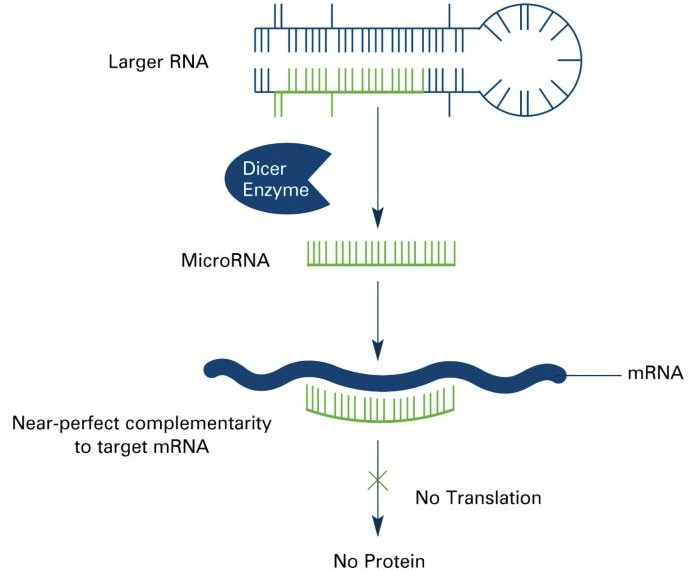
\includegraphics[scale=0.31]{img/mirnas.jpg}
\end{figure}
}
\begin{itemize}
\uncover<2->{
\item Excised by enzymes from longer precursors.
}
\uncover<3->{
\item Precursors folded into hairpin-like secondary structures.
}
\end{itemize}
\end{frame}

\begin{frame}
\frametitle{Background}
\uncover<1->{
MiRNA families
\begin{itemize}
\item Groups of pre-miRNAs based on different criteria (similar ancestry, secondary structure conservation, seed-target relations...)
\item An important aspect used is the analysis of sequence similarity.\\~\\
\end{itemize}
}
\uncover<2->{
Why are they important?
\begin{itemize}
\item Valuable information about biological functions.
\item Amount of information about different miRNAs is variable; families useful for hypothesising characteristics of less known miRNAs.
\item New miRNAs discovered at a fast rate; even low confidence families still useful for researchers (available way before biological validation).
\end{itemize}
}
\end{frame}

\begin{frame}
\frametitle{Introduction}
\uncover<1->{
Project aims
\begin{itemize}
\item Create a computational tool that allows to automatically detect miRNA families from miRBase database (manual process).
\item Establish quality and significance of detected families.
\item Compare different computational approaches and determine the most suitable.\\~\\
\end{itemize}
}
\uncover<2->{
Requirements
\begin{itemize}
\item It was desirable that the tool could predict without human intervention $\rightarrow$ unsupervised machine learning
\item Complete miRBase dataset, so results could be objectively compared to real families in miRBase $\rightarrow$ algorithms able to cluster large datasets
\end{itemize}
}
\end{frame}

\begin{frame}
\frametitle{Methods: Algorithms}
Unsupervised machine learning: Identifies groups of elements based on a similarity measure (obtained by embedded vectors/all-to-all BLAST).\\~\\
\begin{enumerate}
\item<1-> Centroid-based clustering (\textit{k-means++}, Clustal$\Omega$ impl.)\\~\\
\item<2-> Stochastic graph-based clustering (MCL, ref. impl.)\\~\\
\item<3-> Density-based clustering (DBSCAN, scikit-learn impl.)\\
\end{enumerate}
\end{frame}

\begin{frame}
\frametitle{Methods: Statistical validation}

1. Fowlkes-Mallows score\\~\\
External similarity measure, expressed as the geometric mean of the pairwise precision and recall.
\begin{definition}
\begin{equation}
\text{FMS} = \frac{\text{TP}}{\sqrt{(\text{TP} + \text{FP}) (\text{TP} + \text{FN})}}
\end{equation}
\end{definition}
\begin{itemize}
\item TP = true positives\\
\item FP = false posititves\\
\item FN = false negatives
\end{itemize}
\end{frame}

\begin{frame}
\frametitle{Methods: Statistical validation}
2. Adjusted Rand index\\~\\
Similar external similarity measure function, a version of the Rand index corrected for chance.
\begin{definition}
\begin{equation}
\text{RI} = \frac{a + b}{C_2^{n_{samples}}}\ \text{   ;   }
\text{ARI} = \frac{\text{RI} - E[\text{RI}]}{\max(\text{RI}) - E[\text{RI}]}\
\end{equation}
\end{definition}
\begin{itemize}
\item a = true positives
\item b = true negatives
\item \(C_2^{n_{samples}}\) = total number of possible pairs
\item \textit{E}[RI] = expected index of random labellings
\end{itemize}

\end{frame}

\begin{frame}
\frametitle{Results: Data coverage}
\begin{itemize}
\item Ref: 28645 miRNAs in 1983 families in miRBase (69.49\% coverage).
\item About 10\% difference among graph and density-based algorithms.
\item Centroid-based algorithm very different, clusters almost all the sequences.
\end{itemize}
\begin{figure}
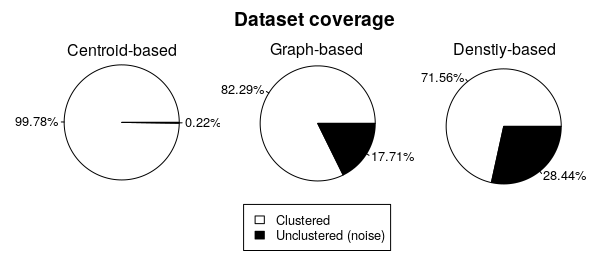
\includegraphics[scale=0.5]{img/coverage.png}
\end{figure}
\end{frame}

\begin{frame}
\frametitle{Results: Quality assessment}
\begin{itemize}
\item Similar patterns observed in FMS and ARI, the former tends to evaluate more positively.
\item The centroid-based algorithm had a much lower score in both.
\item The density-based algorithm had the best score in both measures, followed closely by the graph-based algorithm.
\end{itemize}
\begin{figure}
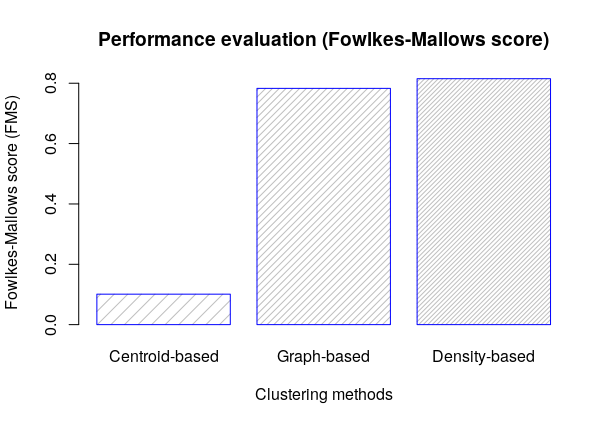
\includegraphics[scale=0.369]{img/fms.png}
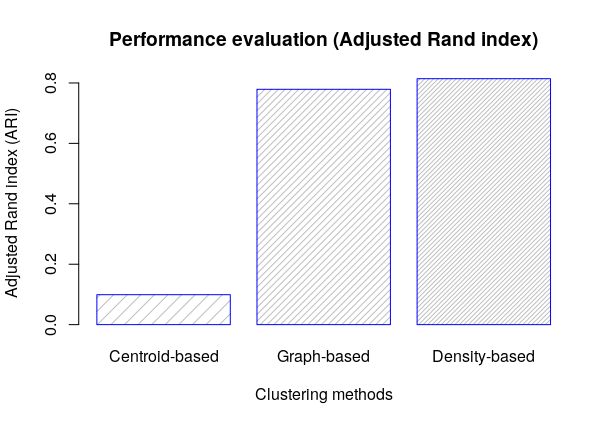
\includegraphics[scale=0.369]{img/ari.png}
\end{figure}
\end{frame}

\begin{frame}
\frametitle{Results: Clustering overview}
\begin{itemize}
\item Low performance of centroid-based algorithm explained by noise sensitivity and hard-wired cluster size threshold in implementation.\\~\\
\item Good performance of graph and density-based algorithms can be explained by their sparse-graph-oriented design.\\~\\
\item Stochastic graph-based algorithm has more coverage and clusters, implementation has better biological data support.\\~\\
\item $\varepsilon$ value parameter in density-based algorithm increases noise detection and improves results.
\end{itemize}
\end{frame}

\begin{frame}
\frametitle{Conclusions}
\begin{itemize}
\item Unsupervised machine learning methods proven very useful for miRNA family detection in large datasets.\\~\\
\item Stochastic graph-based clustering, and specially, density-based clustering are the most suitable.\\~\\
\item The developed tool, miRNACluster, can be effectively used as an automated aid for miRNA family detection or to complement, adjust or improve the miRBase original family predictions.\\~\\
\item The tool is publicly available under an open source license at GitHub (\href{http://www.github.com/samuacosta/miRNACluster}{www.github.com/samuacosta/miRNACluster})
\end{itemize}
\end{frame}

\begin{frame}
\frametitle{}
\begin{center}
\LARGE
Thank you.
\footnotesize
\\~\\
samuel.acostamelgarejo@postgrad.manchester.ac.uk
\end{center}
\footnotesize
\begin{itemize}
\item References:
\begin{itemize}
\tiny
\item Ambros, V. (2004). The functions of animal microRNAs. \textit{Nature}, 431(7006):350–355. Number: 7006 Publisher: Nature
Publishing Group.\\
\item Arthur, D. and Vassilvitskii, S. (2007). k-means++: the advantages of careful seeding. In \textit{Proceedings of the eighteenth annual ACM-SIAM symposium on Discrete algorithms}, SODA ’07, pages 1027–1035, New Orleans, Louisiana. Society for Industrial and Applied Mathematics.
\item Dongen, S., Dongen, v., Hazewinkel, M., and van Eijck, D. (2000). \textit{Graph Clustering by Flow Simulation}. Universiteit Utrecht. Dongen, S., Dongen, v., Hazewinkel, M., and van Eijck, D. (2000). Graph Clustering by Flow Simulation. Universiteit Utrecht.
\item Ester, M., Kriegel, H.-P., Sander, J., and Xu, X. (1996). A density-based algorithm for discovering clusters in large spatial databases with noise. In \textit{Proceedings of the Second International Conference on Knowledge Discovery and Data Mining}, KDD’96, pages 226–231, Portland, Oregon. AAAI Press.
\item Fowlkes, E. B. and Mallows, C. L. (1983). A Method for Comparing Two Hierarchical Clusterings. \textit{Journal of the American Statistical Association}, 78(383):553–569. Publisher: American Statistical Association, Taylor \& Francis, Ltd.
\item Griffiths-Jones, S., Grocock, R. J., van Dongen, S., Bateman, A., and Enright, A. J. (2006). miRBase: microRNA sequences, targets and gene nomenclature. \textit{Nucleic Acids Research}, 34(suppl\_1):D140–D144. Publisher: Oxford Academic.
\item Hubert, L. and Arabie, P. (1985). Comparing partitions. Journal of Classification, 2(1):193–218.
\item Slide 2 image: https://www.genengnews.com/magazine/december-1-2018-vol-38-no-21/microrna-profilers-cite-reconcilable-differences

\end{itemize}
\end{itemize}
\end{frame}


\end{document}
